% !TEX spellcheck = en_US

\documentclass[conference]{IEEEtran}
\usepackage{cite}
\usepackage{amsmath,amssymb,amsfonts}
\usepackage{algorithmic}
\usepackage{graphicx}
\usepackage{textcomp}
\usepackage{xcolor}
% add hyperlinks, delete all .aux files if adding hyperref after previous build
\usepackage{hyperref}
% support for unicode charcters like "é" and "ñ"
\usepackage[T1]{fontenc}
% Provides generic commands \degree, \celsius, \perthousand, \micro and \ohm
\usepackage{gensymb}
% splits a section into multiple columns
\usepackage{multicol}
\def\BibTeX{{\rm B\kern-.05em{\sc i\kern-.025em b}\kern-.08em
    T\kern-.1667em\lower.7ex\hbox{E}\kern-.125emX}}
\begin{document}

\title{Tracker Terrain Loss Part Two}

\author{\IEEEauthorblockN{Mark A. Mikofski}
	\IEEEauthorblockA{DNV, San Diego, CA, 92123, USA }}

\maketitle

\begin{abstract}
Trackers on terrain can incur electric mismatch losses from row-to-row shading, even with backtracking. Standard and slope-aware backtracking algorithms only eliminate row-to-row shade for trackers on flat ground. Tracker terrain loss is the difference between theoretically best performance for trackers on flat ground and the performance for trackers following the terrain, but without any advanced tracking algorithm. We used SolarFarmer to model the Hopewell Friends Solar power plant near Asheboro, NC, which has and average 4\% southwest slope. We calculated a tracker terrain loss of 2.4\% when the entire site is modeled as one layout.
\end{abstract}

\begin{IEEEkeywords}
trackers, terrain, losses
\end{IEEEkeywords}

\section{Introduction}
Write something about \ref{fig:layouts}

\begin{figure}[htbp]
\centerline{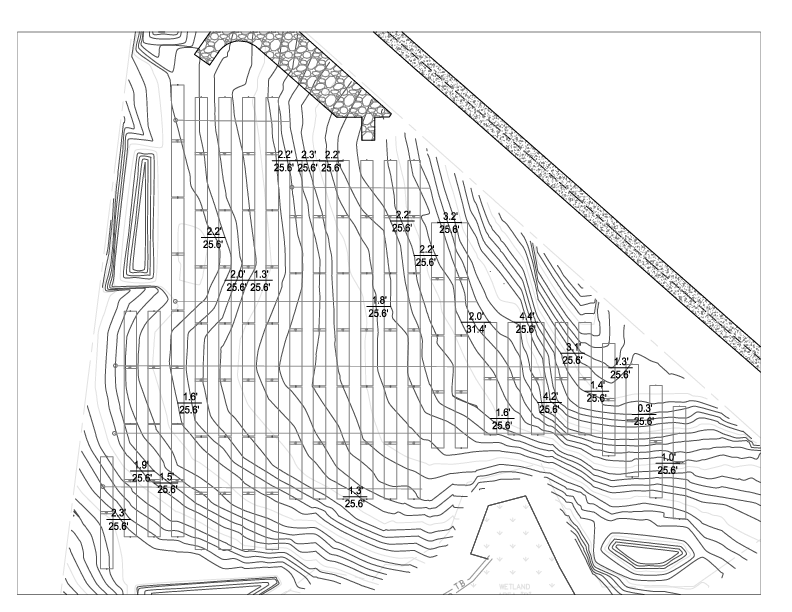
\includegraphics[width=9cm]{Hopewell_Civil_Base.png}}
\caption{Contour map of terrain at Hopewell, NC, single-axis array.}
\label{fig:hopewell_contour_map}
\end{figure}

\begin{figure}[htbp]
\centerline{\includegraphics[width=9cm]{layouts.png}}
\caption{Sketch of 3-layout model, layout \#2 with 30 strings is outlined in red, layout \#1 with 54 strings is to the west and layout \#3 with 27 strings is to the east. The 2-layout model combines layout \#2 and \#3 for 57 strings total, while layout \#1 remains the same.}
\label{fig:layouts}
\end{figure}


Write more stuff and make references to \cite{Marion2013}.

\section{Methods}

\subsection{Model}

Write stuff about SolarFarmer \cite{Mikofski_8547323}.


\subsection{Validation}
This section name doesn't make any sense.

\section{Results}

\subsection{Model Parameters}

\begin{table}[htbp]
\caption{Energy Yield for Tracker Layouts for 5-minute Input Data with Standard Backtracking}
\begin{center}
\begin{tabular}{|c|c|c|c|c|c|}
\hline
\textbf{Lay-}& \textbf{\textit{Terrain}}& \textbf{\textit{GI}}&        \textbf{\textit{Yield}}&        \textbf{\textit{Shading}}& \textbf{\textit{Mismatch}} \\
\textbf{outs}& \textbf{\textit{Mode}}&    \textbf{\textit{$kWh/m^2$}}& \textbf{\textit{$kWh / kW_p$}}& \textbf{\textit{\%}}&      \textbf{\textit{\%}} \\
\hline
1& In Plane& 2044.7&  1695.9& 2.1& 0 \\
 & Follow&         &  1655.8& 2.4& 2.1 \\
\hline
2& In Plane& 2045.9&  1696.2& 2.2& 0 \\
 & Follow&         &  1665.2& 2.3& 1.7 \\
\hline
3& In Plane& 2046.9&  1697.6& 2.2& 0 \\
 & Follow&         &  1670.8& 2.2& 1.4 \\
\hline
\end{tabular}
\label{table:standard-5min}
\end{center}
\end{table}


\begin{table}[htbp]
\caption{Energy Yield for Tracker Layouts for 5-minute Input Data with Slope-Aware Backtracking}
\begin{center}
\begin{tabular}{|c|c|c|c|c|c|}
\hline
\textbf{Lay-}& \textbf{\textit{Terrain}}& \textbf{\textit{GI}}&        \textbf{\textit{Yield}}&        \textbf{\textit{Shading}}& \textbf{\textit{Mismatch}} \\
\textbf{outs}& \textbf{\textit{Mode}}&    \textbf{\textit{$kWh/m^2$}}& \textbf{\textit{$kWh / kW_p$}}& \textbf{\textit{\%}}&      \textbf{\textit{\%}} \\
\hline
1& In Plane& 2045&    1695.9& 2.2& 0 \\
1& Follow&       &    1654.8& 2.4& 2.2 \\
\hline
2& In Plane& 2046.2&  1696.2& 2.2& 0 \\
2& Follow&         &  1664.3& 2.3& 1.7 \\
\hline
3& In Plane& 2047.2&  1697.7& 2.2& 0 \\
3& Follow&         &  1669.8& 2.3& 1.5 \\
\hline
\end{tabular}
\label{table:slope-5min}
\end{center}
\end{table}

\begin{table}[htbp]
\caption{Energy Yield for Tracker Layouts for 1-hour Input Data with Standard Backtracking}
\begin{center}
\begin{tabular}{|c|c|c|c|c|c|}
\hline
\textbf{Lay-}& \textbf{\textit{Terrain}}& \textbf{\textit{GI}}&        \textbf{\textit{Yield}}&        \textbf{\textit{Shading}}& \textbf{\textit{Mismatch}} \\
\textbf{outs}& \textbf{\textit{Mode}}&    \textbf{\textit{$kWh/m^2$}}& \textbf{\textit{$kWh / kW_p$}}& \textbf{\textit{\%}}&      \textbf{\textit{\%}} \\
\hline
1& In Plane& 2048.4&  1700.6& 2.1& 0 \\
 & Follow&         &  1659.1& 2.4& 2.2 \\
\hline
2& In Plane& 2049.9&  1700.9& 2.2& 0 \\
 & Follow&         &  1669.2& 2.3& 1.7 \\
\hline
3& In Plane& 2050.7&  1702.3& 2.2& 0 \\
 & Follow&         &  1675&   2.3& 1.5 \\
\hline
\end{tabular}
\label{table:standard-1hr}
\end{center}
\end{table}


\begin{table}[htbp]
\caption{Energy Yield for Tracker Layouts for 1-hour Input Data with Slope-Aware Backtracking}
\begin{center}
\begin{tabular}{|c|c|c|c|c|c|}
\hline
\textbf{Lay-}& \textbf{\textit{Terrain}}& \textbf{\textit{GI}}&        \textbf{\textit{Yield}}&        \textbf{\textit{Shading}}& \textbf{\textit{Mismatch}} \\
\textbf{outs}& \textbf{\textit{Mode}}&    \textbf{\textit{$kWh/m^2$}}& \textbf{\textit{$kWh / kW_p$}}& \textbf{\textit{\%}}&      \textbf{\textit{\%}} \\
\hline
1& In Plane& 2048.7&  1700.7& 2.2& 0 \\
 & Follow&         &  1658.1& 2.4& 2.2 \\
\hline
2& In Plane& 2050.2&  1701&   2.2& 0 \\
 & Follow&         &  1668.2& 2.3& 1.8 \\
\hline
3& In Plane& 2051.1&  1702.4& 2.2& 0 \\
 & Follow&         &  1674.1& 2.3& 1.5 \\
\hline
\end{tabular}
\label{table:slope-1hr}
\end{center}
\end{table}
\subsection{Validation Metrics}

\section{Conclusions}
Write the conclusions.

\section*{Acknowledgment}

Data and layout specifications for the Hopewell, NC solar array were provided by PV Evolution Labs and Cypress Creek Renewables based on funding by the U.S. Department of Energy, Energy Efficiency and Renewable Energy as detailed in the funding opportunity announcement, DE-FOA-0001840 \cite{CypressCreekRenewables2019}.

\bibliographystyle{IEEEtran}
% argument is your BibTeX string definitions and bibliography database(s)
\bibliography{IEEEabrv,bibliography}

\end{document}
